\documentclass[12pt]{article}
\usepackage[utf8]{inputenc}
\usepackage{float}
\usepackage{amsmath}
\usepackage{blkarray}
\usepackage{tikz}


\usepackage[hmargin=3cm,vmargin=6.0cm]{geometry}
%\topmargin=0cm
\topmargin=-2cm
\addtolength{\textheight}{6.5cm}
\addtolength{\textwidth}{2.0cm}
%\setlength{\leftmargin}{-5cm}
\setlength{\oddsidemargin}{0.0cm}
\setlength{\evensidemargin}{0.0cm}

\begin{document}

\section*{Student Information } 
%Write your full name and id number between the colon and newline
%Put one empty space character after colon and before newline
Full Name : Mehmet Rüçhan Yavuzdemir \\
Id Number : 2522159 \\

% Write your answers below the section tags
\section*{Answer 1}
\subsection*{a) }
By the Handshaking Theorem, sum of degrees of all nodes equal to $2 \cdot|E| = 2 \cdot 7 = \textbf{14}$. Alternatively, we can sum all the degrees up, 3+3+3+3+2 = \textbf{14}.

\subsection*{b) }

Let R be adjacency list representation of G.\\

R = 
$\begin{pmatrix} 
0&1&1&0&1\\
1&0&1&0&1\\
1&1&0&1&0\\ 
1&0&1&0&0\\
1&1&0&1&0\\
\end{pmatrix}$
\\\\
Hence, there are \textbf{14} non-zero values.

\subsection*{c) }
Let R be the incident matrix representation of G. \\
\begin{matrix} 
R =
\end{matrix}\,
\bordermatrix{     
    & e_1&e_2&e_3&e_4&e_5&e_6&e_7\cr
    a&1&0&0&0&1&1&0\cr
    b&1&1&0&0&0&0&1\cr
    c&0&1&1&0&0&1&0\cr
    d&0&0&1&1&0&0&0\cr
    e&0&0&0&1&1&0&1\cr
}
\\\\
Hence, there are \textbf{21} zeros.

\subsection*{d) }
To have a complete graph with 4 vertices, we should have 4 vertices with all degrees 3. However, to have 4 vertices graph, we should remove vertex d. Although we have 4 vertices with degree 3, we still do not have a possible complete graph. If we select 5 vertices, there should be 5 vertices with degree 4, which is not the case. If we had c-e edge, we would have a complete graph with 4 vertices; a, b, c, e. But in this case, \textbf{there is no such a subgraph}.

\subsection*{e) }
If we can color the graph with only two colors, with the constraint that adjacent vertices should have different colors, the graph is bipartite. Else, G is not bipartite. Let's assume we have white and black colors.

Let a be painted with white, then b, c and e should be black since they are neighbours of a. However, there exists an edge between b and c, this contradicts our constraint. They cannot be in the same color. \textbf{Hence, G is not bipartite.}\\ 

\subsection*{f) }

There are 7 undirected edges. If we convert this graph into an directed graph that have G as its underlying undirected graph, we would have a 2 decisions for each edge. Hence, we have \textbf{$2^7 = 128$} directed graphs.

\subsection*{g) }
A simple path is a path that does not include repeating vertices. Since we have 5 vertices, we can have a simple path with at most 4 edges. For example, \textbf{b-c-d-e-a} is an example of the longest simple path. Hence, our answer is \textbf{4}.

\subsection*{h) }
Let u and v be any the vertices in G. There are always a path between them in since graph G is a connected graph. There are no seperated other graphs and components left. Hence, G has only \textbf{1} connected component. 

\subsection*{i) }
An Euler circuit is a cycle that starts and ends at the same vertex and visits all the edges exactly once. The necessary condition for having an Euler circuit is that all vertices should have even degrees. If we find a vertex with an odd degree, by the definition of the Euler circuit, we can conclude that there is no Euler circuit in G. \\\\

Since $deg(v_a) = deg(v_b) = deg(v_c) = deg(v_e) = 3$, graph G does \textbf{not} have any Euler circuit.

\subsection*{j) }

An Euler path is a trail that visits all the edges exactly once. The necessary condition for having an Euler path is that there should be zero or two vertices with odd degrees. If we find a contradiction, by the definition of the Euler path, we can conclude that there is no Euler path in G. \\\\

Since $deg(v_a) = deg(v_b) = deg(v_c) = deg(v_e) = 3$, $4 \neq 0$ and $4 \neq 2$, graph G does \textbf{not} have any Euler path.

\subsection*{k) }

A Hamilton circuit is a cycle that starts and ends at the same vertex and visits all the vertices exactly once. \\\\

The cycle \textbf{b-c-d-e-a-b} is an example of a Hamilton circuit since it visits all the vertices exactly once. 

\subsection*{l) }

A Hamilton path is a trail that visits all the vertices exactly once. \\\\

The path \textbf{b-c-d-e-a} is an example of a Hamilton path since it visits all the vertices exactly once. 

\section*{Answer 2}

The function f with $f(a) = a',$ $f (b) = b',$ $f (c) = c',$ $f(d) = d'$ and $f(e) = e'$ is a one-to-one correspondence between the vertices of the graphs G and H according to their degrees. Hence, G and H are isomorphic.

Alternatively,  we can see these edges in their adjacency matrix:

\begin{equation}
\begin{matrix} 
G_E = 
\end{matrix}\,
\bordermatrix{     
    & a&b&c&d&e\cr
    a&0&1&0&0&1\cr
    b&1&0&1&0&0\cr
    c&0&1&0&1&0\cr
    d&0&0&1&0&1\cr
    e&1&0&0&1&0\cr
}
\end{equation}
\begin{equation}
\begin{matrix} 
H_E = 
\end{matrix}\,
\bordermatrix{     
    & a'&b'&c'&d'&e'\cr
    a'&0&1&0&0&1\cr
    b'&1&0&1&0&0\cr
    c'&0&1&0&1&0\cr
    d'&0&0&1&0&1\cr
    e'&1&0&0&1&0\cr
}
\end{equation}
\\Since $G_E$ and $H_E$ are identical, G and H are isomorphic.

\section*{Answer 3}

For the Dijkstra's Algorithm, all we have to do is start by the source node. \\

At each step, we will choose the non-visited node that has minimum distance, and explore its non-visited neighbours. Update the distance if new possible distance is smaller than the current distance.\\

We will denote a visited vertex by putting an apostrophe after it.\\

\noindent \begin{matrix} 
distance =
\end{matrix}\,
\bordermatrix{     
    & s&u&w&v&x&y&z&t\cr
    &\infty&\infty&\infty&\infty&\infty&\infty&\infty&\infty\cr
} 
All distances are set to $\infty$.\\
\begin{matrix} 
distance = 
\end{matrix}\,
\bordermatrix{     
    & s&u&w&v&x&y&z&t\cr
    &0&\infty&\infty&\infty&\infty&\infty&\infty&\infty\cr
}
s set to 0 since it is the source node.\\
\begin{matrix} 
distance = 
\end{matrix}\,
\bordermatrix{     
    & s'&u&w&v&x&y&z&t\cr
    &0&4&3&5&\infty&\infty&\infty&\infty\cr
}
mark s as visited and explore its neighbours\\
\begin{matrix} 
distance = 
\end{matrix}\,
\bordermatrix{     
    & s'&u&w'&v&x&y&z&t\cr
    &0&4&3&5&11&\infty&15&\infty\cr
}
mark w as visited and explore its neighbours\\
\begin{matrix} 
distance = 
\end{matrix}\,
\bordermatrix{     
    & s'&u'&w'&v&x&y&z&t\cr
    &0&4&3&5&11&15&15&\infty\cr
}
mark u as visited and explore its neighbours\\
\begin{matrix} 
distance = 
\end{matrix}\,
\bordermatrix{     
    & s'&u'&w'&v'&x&y&z&t\cr
    &0&4&3&5&7&11&15&\infty\cr
}
mark v as visited and explore its neighbours\\
\begin{matrix} 
distance = 
\end{matrix}\,
\bordermatrix{     
    & s'&u'&w'&v'&x'&y&z&t\cr
    &0&4&3&5&7&8&13&\infty\cr
}
mark x as visited and explore its neighbours\\
\begin{matrix} 
distance = 
\end{matrix}\,
\bordermatrix{     
    & s'&u'&w'&v'&x'&y'&z&t\cr
    &0&4&3&5&7&8&12&17\cr
}
mark y as visited and explore its neighbours\\
\begin{matrix} 
distance = 
\end{matrix}\,
\bordermatrix{     
    & s'&u'&w'&v'&x'&y'&z'&t\cr
    &0&4&3&5&7&8&12&15\cr
}
mark z as visited and explore its neighbours\\
\begin{matrix} 
distance = 
\end{matrix}\,
\bordermatrix{     
    & s'&u'&w'&v'&x'&y'&z'&t'\cr
    &0&4&3&5&7&8&12&15\cr
}
mark t as visited and explore its neighbours\\

Hence, shortest path from s to t is : \textbf{s-v-x-y-z-t} with cost 15.
\section*{Answer 4}
\subsection*{a) }

For this question, we are going to make use of Kruskal's algorithm, which is a Greedy algorithm. At each step, we will choose the edge with the lowest weight. If the new edge would cause a cycle, we skip it. Let's sort the edge weights.

2 2 2 2 3 3 3 4 4 4 4 5 5 5 5 ... \\\\

For the spanning tree, we should have $|V|-1$ edges. There are 11 vertices, which means that to avoid a cycle, we should select 10 edges, and include all 11 vertices.\\

We can select the edges in this order:\\\\

(2)(b-c), (2)(c-f), (2)(h-i), (2)(d-k), (3)(a-b), (3)(c-d), (3)(f-j), (4)(e-f), (4)(f-i) (4)(f-g).\\\\

We selected 10 edges, and any of them cause a cycle, so we are done.

\subsection*{b) }

\begin{figure}[H]
	\centering
	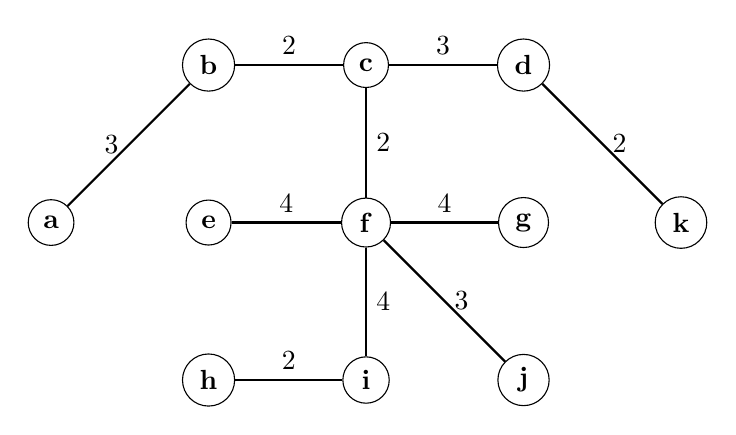
\begin{tikzpicture}
	
	\node[shape=circle,draw=black] (a) at (-2, 2)     {\textbf{a}};
	\node[shape=circle,draw=black] (b) at (0, 4)     {\textbf{b}};
	\node[shape=circle,draw=black] (c) at (2, 4)     {\textbf{c}};
	\node[shape=circle,draw=black] (d) at (4, 4)     {\textbf{d}};
	\node[shape=circle,draw=black] (e) at (0, 2)     {\textbf{e}};
	\node[shape=circle,draw=black] (f) at (2, 2)     {\textbf{f}};
	\node[shape=circle,draw=black] (g) at (4, 2)     {\textbf{g}};
	\node[shape=circle,draw=black] (h) at (0, 0)     {\textbf{h}};
	\node[shape=circle,draw=black] (i) at (2, 0)     {\textbf{i}};
	\node[shape=circle,draw=black] (j) at (4, 0)     {\textbf{j}};
	\node[shape=circle,draw=black] (k) at (6, 2)     {\textbf{k}};
	
	\path[-, thick] (a) edge node[left]{3} (b);
	\path[-, thick] (b) edge node[above]{2} (c);
	\path[-, thick] (c) edge node[above]{3} (d);
	\path[-, thick] (c) edge node[right]{2} (f);
	\path[-, thick] (d) edge node[right]{2} (k);
	\path[-, thick] (e) edge node[above]{4} (f);
	\path[-, thick] (f) edge node[above]{4} (g);
	\path[-, thick] (f) edge node[right]{4} (i);
	\path[-, thick] (f) edge node[right]{3} (j);
	\path[-, thick] (h) edge node[above]{2} (i);
	
	\end{tikzpicture} 
	\label{fig:g4}
\end{figure}


\subsection*{c) }

No, the spanning tree is not unique because there is still an unused edge that doesn't cause any cycle and can be used in another minimum spanning tree. For example, if we change the (4)(f-g) edge with the (4)(g-j) edge, we have again a minimum spanning tree. Notice that they have the same weight. Hence, the minimum spanning tree is not unique.


\end{document}
